\subsection{Encountered problems}\label{subsec:encountered-problems}

\TODO {
    Talk about certain difficulties where did I need to find the workarounds where something was not straightforward.
}

During the development two major difficulties were encountered which we are discussed in this section.

The first problem is related to the analysis model of the SonarQube.
Currently, SonarQube assumes that all of the code smells can be detected during a single
analysis of a node.
The issue is that a big number of code smells implemented by us require context of other nodes.
For example, in order to find cyclic dependencies, we first need to detect all of the dependencies
of a class and then, after all of the dependencies of all of the classes inside of the application have been detected,
we would transform the dependencies into a graph and look for the cycles in the graph.

Fortunately, SonarQube provides a possibility to implement sensors, which can fully control the execution flow
of the analysis.
By using sensors, we were able to create a custom execution pipeline for the rules that require context of the project
and not just a single node.
This approach allowed us to solve the original problem, but lead to another one.

The second problem is related to the API that SonarQube plugin base exposes.
As mentioned in section~\ref{subsec:sonarqube-plugin-development}, we followed the guide provided by the SonarQube community in
order to implement our plugin.
This includes the usage of the base dependency which includes the API for accessing the AST generated by SonarQube.
Not only that, but this dependency also contains other utilities, such as various visitors which can be used to detect
various measures inside the code such as complexity or count the lines of code.
But the problem is that those some classes are available only during the compile time of the application and
are missing from the runtime, inside which the plugin is loaded during analysis execution.

As mentioned previously, we used sensors to implement the pipeline for the rules that have state.
But the sensor pipeline is fully custom as the input that you receive are source files of the project and not
parsed AST as it is with normal rules.
This means that you need to parse the files into the AST by yourself and it was not that simple to do due to the some
of the classes missing from the runtime.

One of the solutions could be to include the full library inside the compiled artifact and bring all those classes with
the plugin itself.
But this would mean that you would also bring the implementations of the AST tree nodes and this would cause
\verb|ClassCastException|-s at runtime of the plugin because of how Java Virtual Machine (JVM) handles classes loaded
by different class loaders: even though the classes are effectively the same if they were loaded by the different class loaders
JVM cannot guarantee that they are indeed the same, so casting between those types is not allowed.

In order to fix this issue, a fork was created out of the plugin base dependency and all of the classes
that are exposed by the API were left out of it, in order to fix aforementioned problem with class loaders.
Then we could use this include our own dependency to parse the input files to AST the same way SonarQube would do it
and also use all of the utilities that are present in the SonarQube base dependency for our own needs.

The library is also open source and can be found in the Github repository~\cite{sonar_java_extracted}.

\subsection{Issues and limitations}\label{subsec:issues-and-limitations}

\TODO{
    Point out some limitations that I wanted to do but are still missing
}

After the implementation has been completed, there are still some issues that we would like to fix in the future.

Firstly, some of the rules have been implemented as normal SonarQube rules, when they should be actually implemented
as sensor rules.
A great example would be \verb|Shotgun surgery|.
This rule was implemented as a regular SonarQube rules although it has state and this results in a situation where
we have to check for issues after every scanned class because we never know whether or not this class is the last that
we would scan.
This was implemented so because the implementation of the rule was done before we developed the internal sensor \say{framework}
and there was no reason to rewrite it because it works the way it is implemented now.
Nonetheless, it would be more efficient to rewrite this rule as a sensor rule.

Secondly, we did not have time to implement nice descriptions for the rules.
SonarQube UI provides a possibility to include a description for the rule that the user would read in order
to understand the idea behind the rule and also see compliant / non-compliant code examples as it can be seen
in figure~\ref{fig:sonarqube_description_example}.

\begin{figure}
    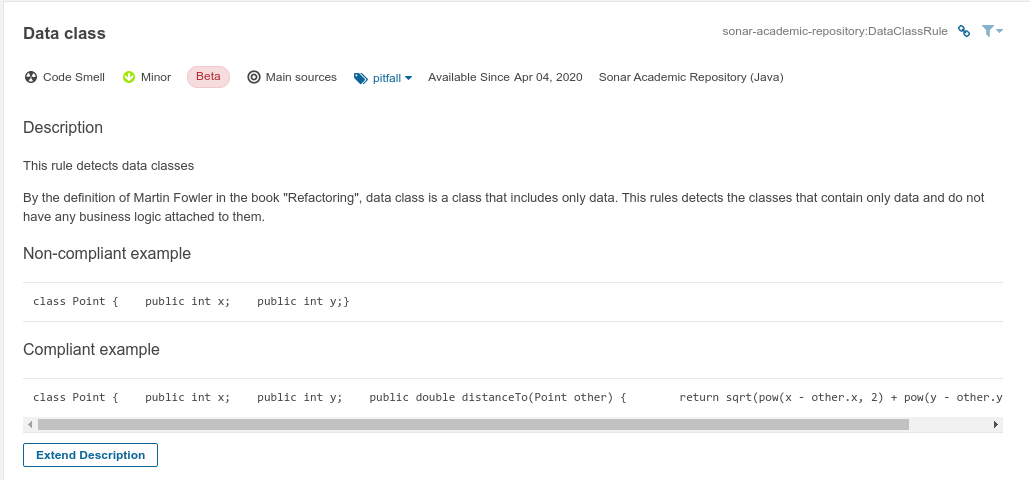
\includegraphics[scale=0.45]{figures/sonarqube_description.png}
    \caption{SonarQube rule description example.}
    \label{fig:sonarqube_description_example}
\end{figure}

Currently we assume that the user is familiar with the rules and does not require any assistance in understanding how
a given rule works, but it would still be nice to have complete and concise descriptions about rule implementations.

Finally, there as an issue with threshold calculation that has been mentioned in section~\ref{subsec:analysis-results}.
Some of the thresholds were not calculated by us, so they might be drastically different for Java applications from
Swift applications.

\FloatBarrier

\subsection{Result validity}\label{subsec:result-validity}

\TODO {
    Talk about the analysis results:
    \begin{itemize}
        \item Compare with another paper
        \item Take only code smells that are only in that table and compare their and results (paretto chart) (guess the values)
        \item Ignore the blue one (because this is desktop)
        \item It would be nice if the results are not tha different (gives some confidence that our calculations make sense), but we can analyze much more
    \end{itemize}
}

\subsection{Potential usages}\label{subsec:potential-usages}

\TODO{
    In this section, we should describe how external users can use our tool.
    We can focus on 3 groups that we will introduce in introduction.
    Developers, project managers and data scientist?
    For each group, we can write a section and describe how they can use the tool and see useful
    information about the projects.
}

\subsubsection{Developers}

\TODO{
    Think of how this tool is useful for developers.
    Obviously this is the main focus group.
}

\TODO{
    Developers can use this tool for statical analysis of the application they develop.
    Here we can show detailed view of a single code smell, with message line
    and rule description and "ideas" on how to fix the bug in the rule description.
}

\subsubsection{Project managers}

\TODO{
    Project managers can see the overview of the project and how
    much code smells there are in the project.
    Also they can see how many of each rule, etc.
    Here we can show general view of the project (the dashboard).
}

\subsubsection{Data scientists}

\TODO{
    How can the data scientists use this?
    In general, they can export datasets from SonarQube like we did.
    Perhaps we can describe here how we did this, and what we managed to create (e.g. analysis results).
    With this, they can perhaps find correlations if different code smells can be usually found together.
}
